To find out what parts of Personal Informatics that apply to the field of telehealth and what new parts that arise, we conducted interviews with six COPD-patients that used the AmbuFlex telehealth system. We here bring the Activity Plan developed prior to conducting the interviews. The results from the interviews are presented in the paper.

%This chapter serves as extended documentation to the paper, were we bring the results. 

All interviews are audio recorded and the recordings can be found on attached CD.

\section{Activity Plan}
We dedicate one hour for each of the interviews. Two researchers are present during the interviews, one will facilitate the interview and an observer is responsible for audio and taking notes.  The interviews will be conducted as semi-structured interviews. Questions will relate to the use and the experience of the telehealth system. The interview also include the patient showing how to use the system, which the researchers will observe to find any potential user needs.

\textbf{Agenda}
\begin{itemize}
	\item Consent form (included on attached CD)
	\item Interview
	\item Observe use of telehelath system
\end{itemize}

A signed consent form is a prerequisite to the interviews.

\textbf{Interviews}

Demographics:
\begin{itemize}
	\item How old are you?
	\item Do you live alone?
	\item Do you have other diseases?
	\item What are your experience with technologies/iPad/tablets/smartphones?
\end{itemize}

COPD-related:
\begin{itemize}
	\item Which degree of COPD do you have?
	\item Can you explain to me, how it is to have COPD?
	\item Have you experienced anxiety related to your COPD?
	\begin{itemize}
		\item In what situations are you more anxious than others?
	\end{itemize}
	\item How many exacerbations have you experienced? Describe the experience to me.
\end{itemize}


Self-management:
\begin{itemize}
	\item How do you manage COPD?
	\item Do you receive home care?
	\item Do you receive any help from relatives or friends?
	\item Do you smoke?
	\item Have you attended any rehabilitation programs? If yes, which? If no, why not?
	\item Have you attended education at Lungeskolen? If yes, has it helped you manage your COPD and how?
	\item Do you consider your diet?
	\item Is physical activity a part of your rehabilitation?
	\item Do you have a care plan? Do you use it? Why (not)?
	\begin{itemize}
		\item What have you used it for? Or how have you used it?
	\end{itemize}
	\item When do you take your medication?
\end{itemize}

Telehealth system:
\begin{itemize}
	\item How often do you measure?
	\item What motivates you to measure?
	\item What happens when you have entered your measures?
	\item When are your entries monitored?
	\item How is the dialogue between you and your nurse?
	\item Do you assess you measures yourself?
	\begin{itemize}
		\item For an exacerbation? If so, do you initiate medication yourself?
		\item Do you wait for answer from the monitoring before initiating medication?
	\end{itemize}
	\item How is the waiting time after you have submitted your measures until you get a response from the monitoring?
	\item Are you familiar with your measures' recommended level?
	\begin{itemize}
		\item Would you like to know them?
	\end{itemize}
	\item How has telehealth helped you in managing your COPD?
	\begin{itemize}
		\item Has telehealth made it easier to recognise day-to-day variations?
		\item Has telehealth made it easier to recognise an exacerbation?
	\end{itemize}
	\item Do you learn anything about your COPD from using the telehealth system?
	\item Do you reflect on your measures?
	\item What problems have you experienced from using telehealth?
	\item What symptoms do you experience related to COPD? Do you experience the symptoms that the system cover?
	\begin{itemize}
		\item Is it easy to answer yes/no to "Do you cough more than usual?"
	\end{itemize}
	\item What do you gain from using telehealth?
	\begin{itemize}
		\item Do you feel secure? Why?
		\item What is needed for you to feel more secure?
	\end{itemize}
	\item When are you in doubt?
	\item Are there any concrete situations where you get confused?
	\item What do you think is hard?
	\item Can you show me how you use the telehealth system?
\end{itemize}



\section{Own tracking system}

As presented in the paper, two of the six patients did parallel tracking on paper as AmbuFlex does not provide access to past measures. One example, can be seen on figure \ref{fig:paperSystem}.

\begin{figure}[h]
\centering
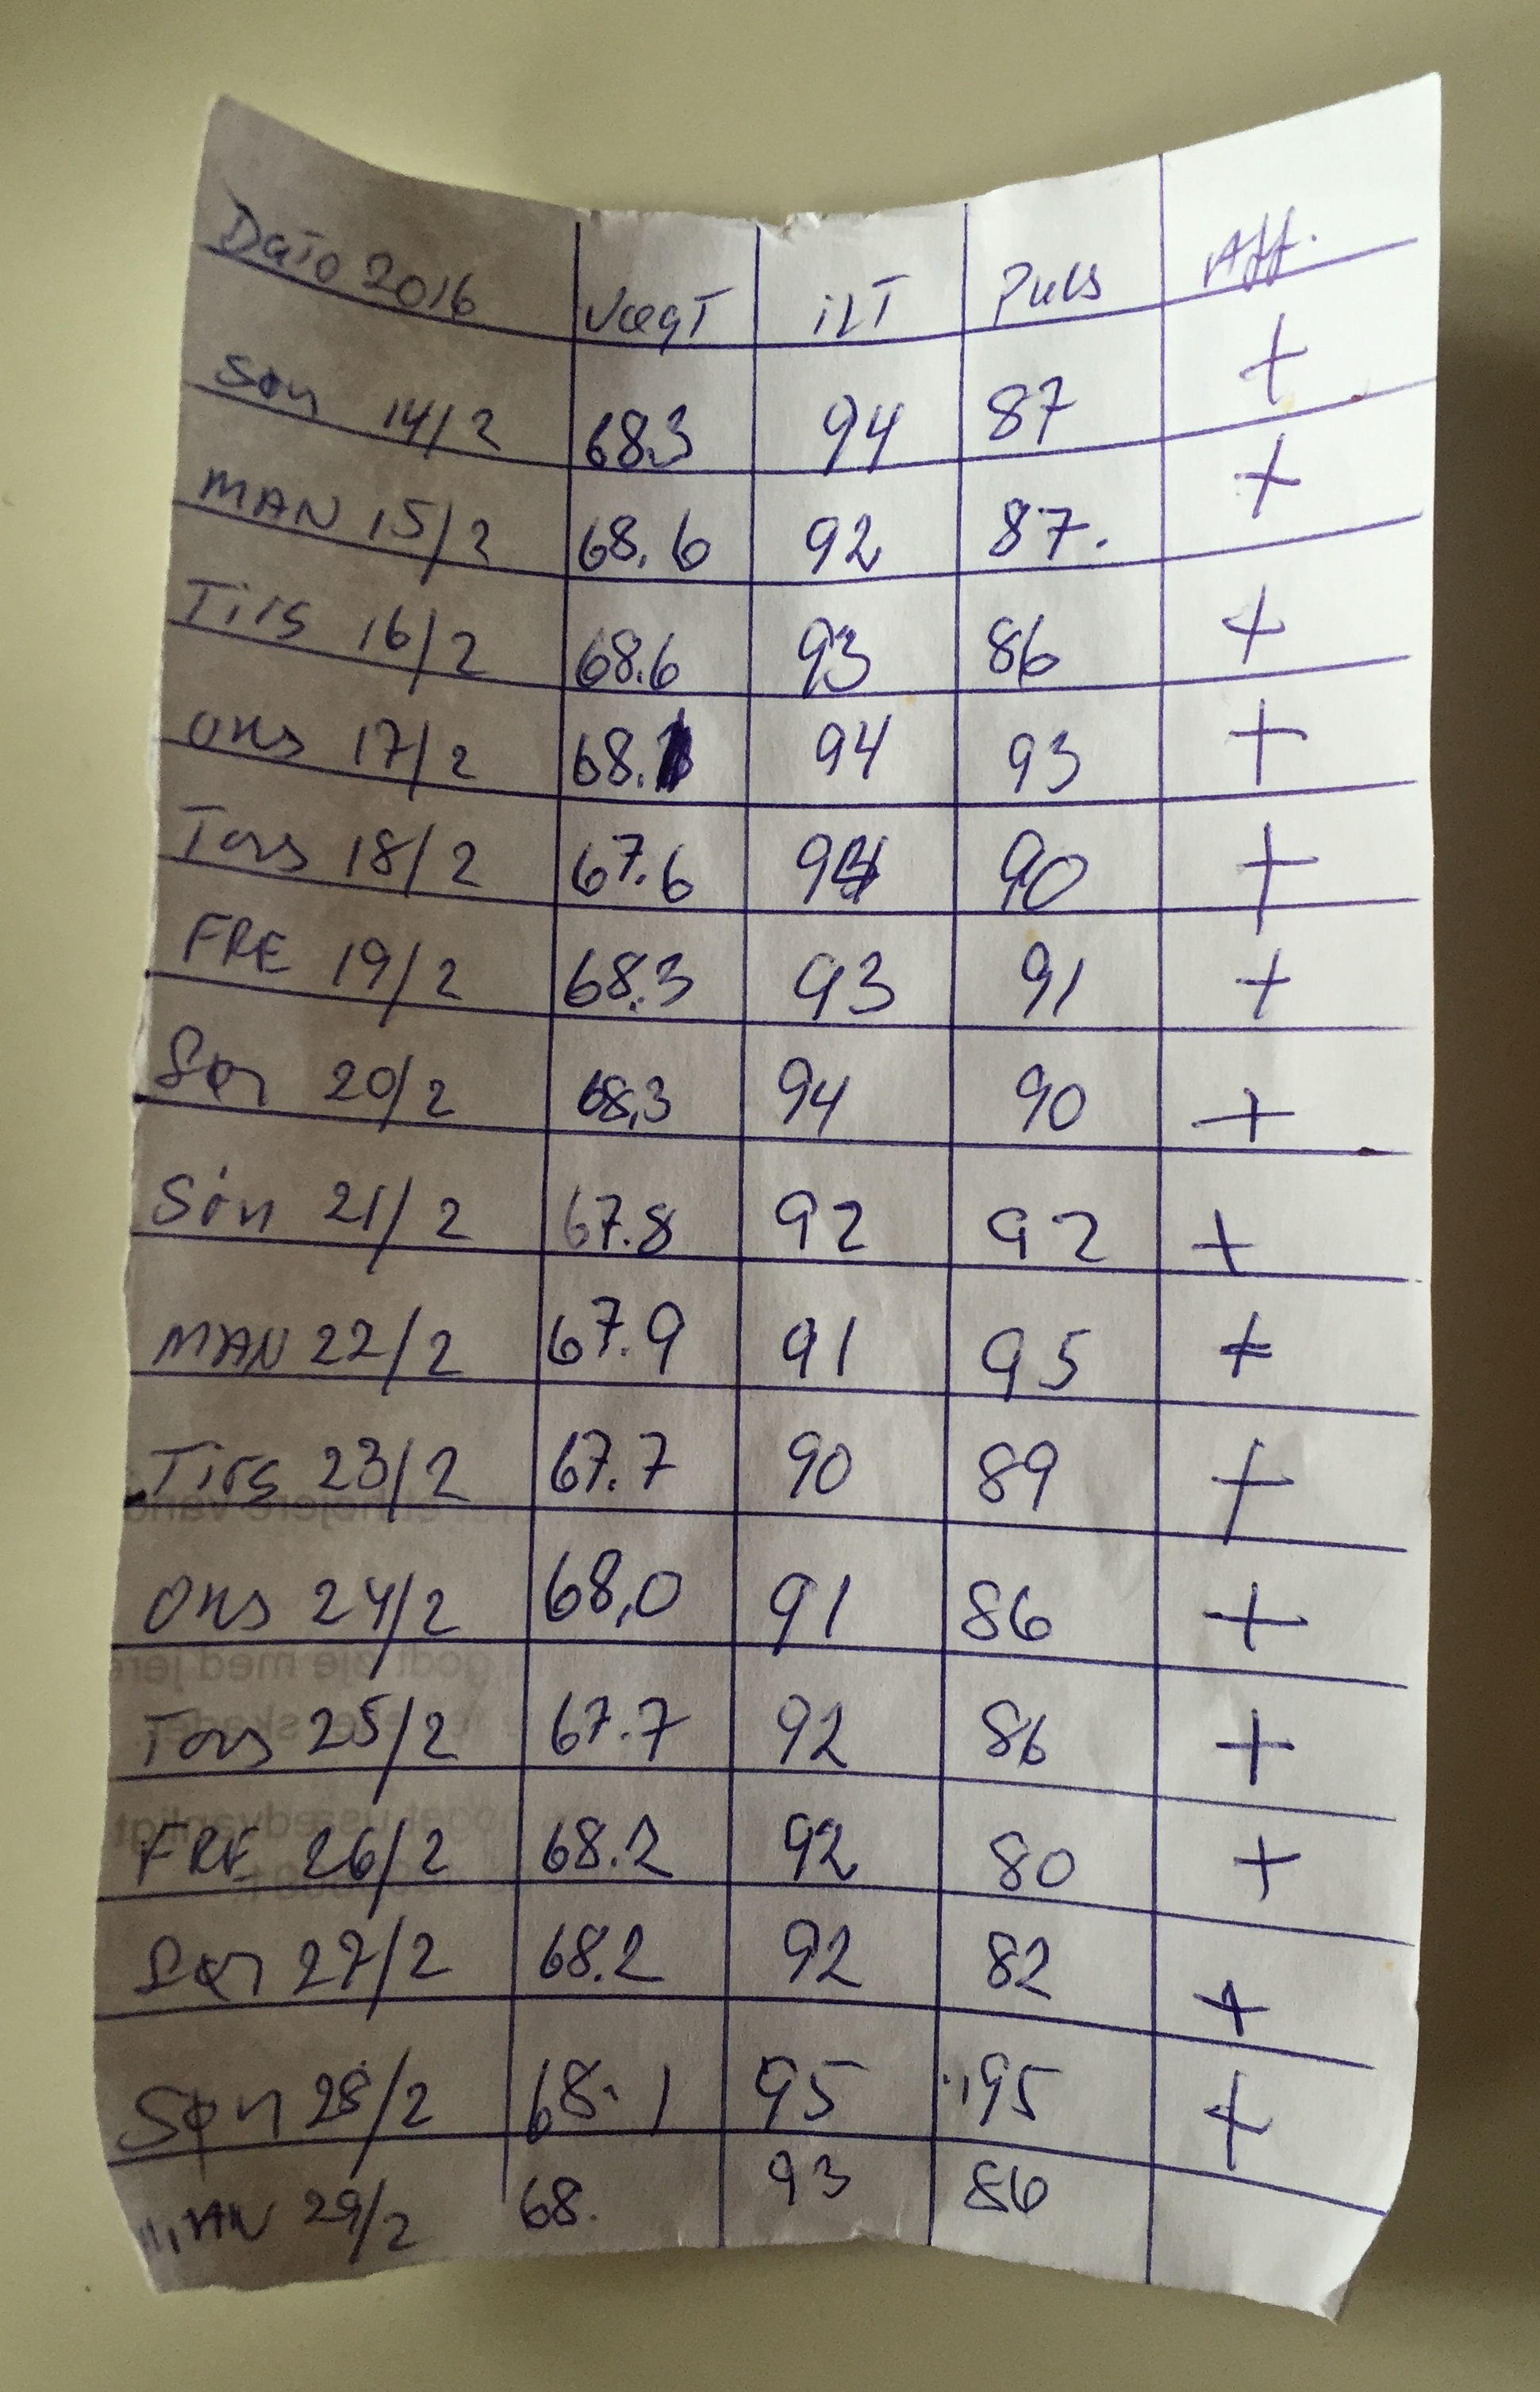
\includegraphics[scale=0.09]{images/study1/prebens.png}
\caption{A parallel tracking system developed by a spouse to one of the patients.}
\label{fig:paperSystem}
\end{figure}

Besides tracking the measures from AmbuFlex this tracking system also include another variable that was found relevant by the patient and the patient's spouse themselves.

%\includepdf[pages=-, pagecommand={}]{Appendices/Aktivitetsplan.pdf}